\section{Конструкторский раздел}

В данном разделе приведены ключевые алгоритмы использовавшиеся при написании драйвера и демона.

\subsection{Структура ПО}

Разрабатываемое ПО состоит из драйвера геймпада в виде загружаемого модуля ядра, и демона, запускаемого с использованием утилиты \texttt{systemd} \cite{systemd}. Структура ПО представлена на рисунке \ref{fig:po-struct}.

\begin{figure}[ht]
    \centering
    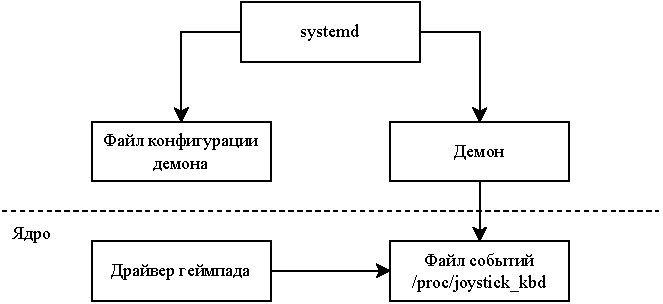
\includegraphics[width=\linewidth]{img/po-structure.pdf}
    \caption{Структура ПО}
    \label{fig:po-struct}
\end{figure}

\clearpage

\subsection{Последовательность преобразований}

\begin{figure}[ht]
    \centering
    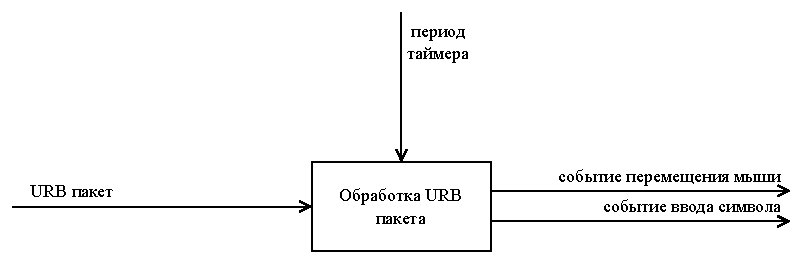
\includegraphics[width=\linewidth]{img/idef0-A0.pdf}
    \caption{IDEF0-диаграмма процесса обработки URB пакета. (Часть 1)}
\end{figure}

\begin{figure}[ht]
    \centering
    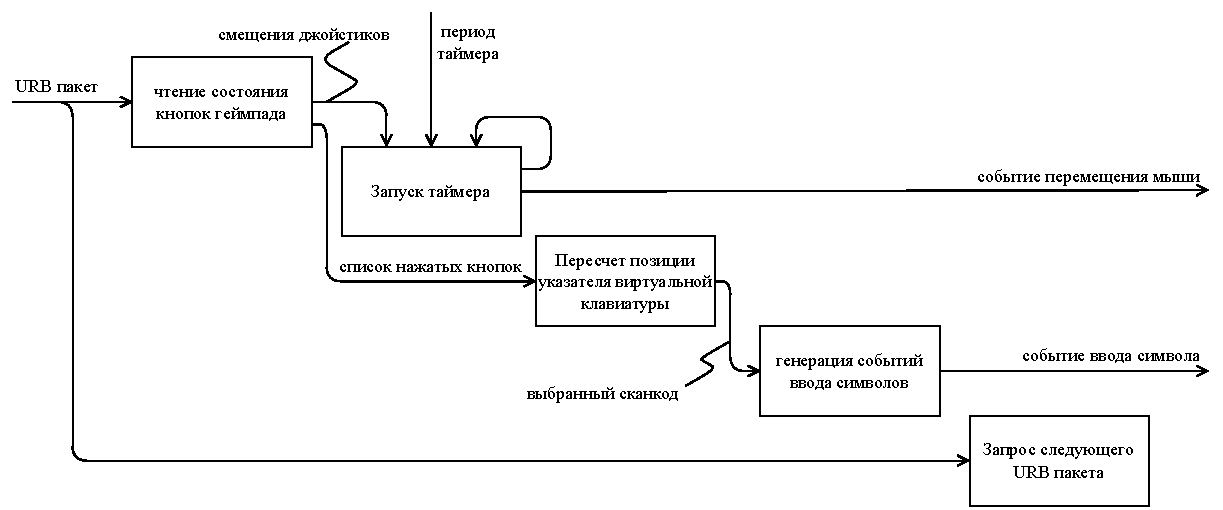
\includegraphics[width=\linewidth]{img/idef0-A1.pdf}
    \caption{IDEF0-диаграмма процесса обработки URB пакета. (Часть 2)}
\end{figure}

\subsection{Алгоритм обработки URB}

\begin{figure}[ht]
    \centering
    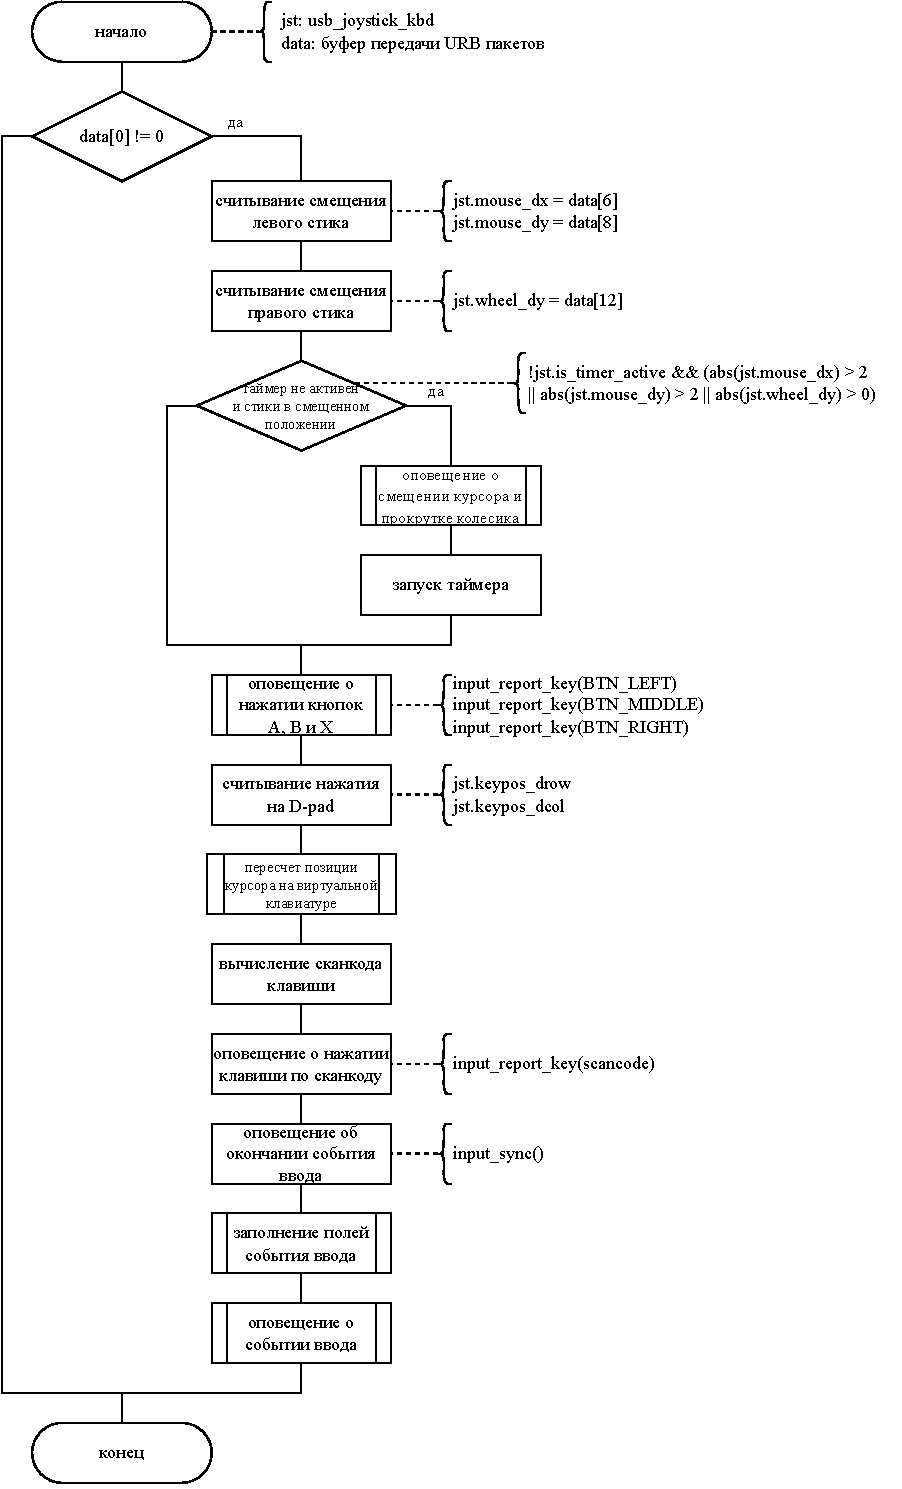
\includegraphics[keepaspectratio,width=\linewidth,height=0.85\textheight]{img/urb-handle.pdf}
    \caption{Алгоритм обработки URB пакета}
    \label{alg:urb-handle}
\end{figure}

\clearpage

\subsection{Алгоритм генерации события перемещения указателя}

На рисунке \ref{alg:emit-event} представлен алгоритм генерации события с пробуждением ждущих процессов.

\begin{figure}[ht]
    \centering
    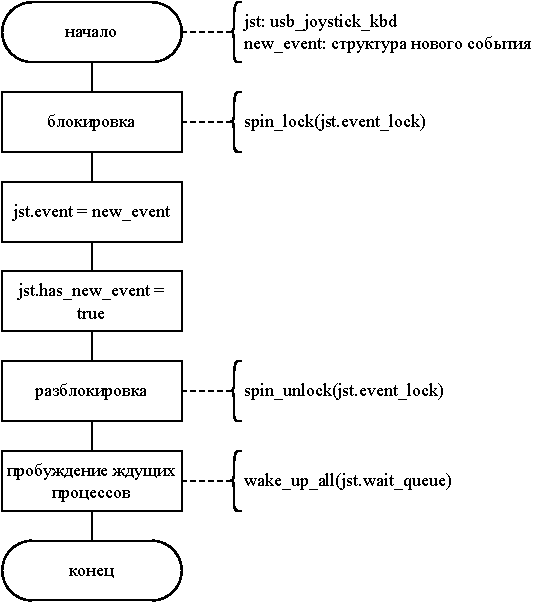
\includegraphics[keepaspectratio,width=0.75\linewidth,height=0.85\textheight]{img/emit-event.pdf}
    \caption{Алгоритм генерации события перемещения указателя виртуальной клавиатуры}
    \label{alg:emit-event}
\end{figure}

\subsection{Алгоритм чтения события перемещения указателя}

На рисунке \ref{alg:proc-read} приведен алгоритм чтения события с блокировкой и ожиданием.

\begin{figure}[ht]
    \centering
    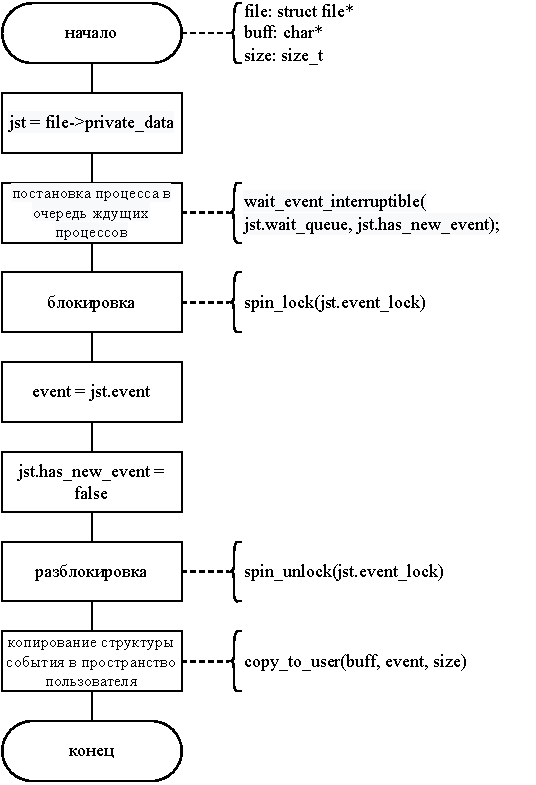
\includegraphics[keepaspectratio,width=\linewidth,height=0.85\textheight]{img/proc-read.pdf}
    \caption{Алгоритм чтения события из файла}
    \label{alg:proc-read}
\end{figure}

% TODO: алгоритм воркера в демоне

\pagebreak
